% intensity
% spectral distribution
% solar geometry
% saules stāvoklis debesīs
% un virziens, kurā stara starojums krīt uz dažādu virzienu un ēnojuma virsmām

Lielākā daļā Saules emitētās enerģijas tiek saražota kodolreakcijās fotosfērā.

Solārā konstante $G_{sc}$ ir saņemtā enerģija laika vienībā uz laukuma vienības perpendikulāri starojuma izplatīšanās virzienam 1 AU attālumā integrēta pa visiem viļņu garumiem.\cite{ThermalProcesses}



TIM (Total Irradiance Montior) in SORCE (SOlar Radiation and Climate Experiment) of NASA 
daily measurement from feb 2003 until present


Kopējais saules apstarojums (TSI) ir saules starojuma absolūtās intensitātes mērījums integrēts visā saules enerģijas diskā un visā saules enerģijas spektrā.

diennakts vidējais apstarojums 1 AU attālumā no Saules.

Norāda uz solārās radiācijas izmaiņām, kas ietekmē solārās enerģijas apjomu uz Zemes atmosfēras augšējiem slāņiem.


Šajā darbā tiek izmantot TSI dati no SORCE (SOlar Radiation and Climate Experiment) TIM (Total Irradiance Montior) dati, pēc kuriem absolūtā vērtība ir $1360.8 \pm 0.5 \textrm{Wm}^{-2}$, jo tie ir precīzākie un ...\cite{Frohlich2012}

\begin{figure}
    \centering
    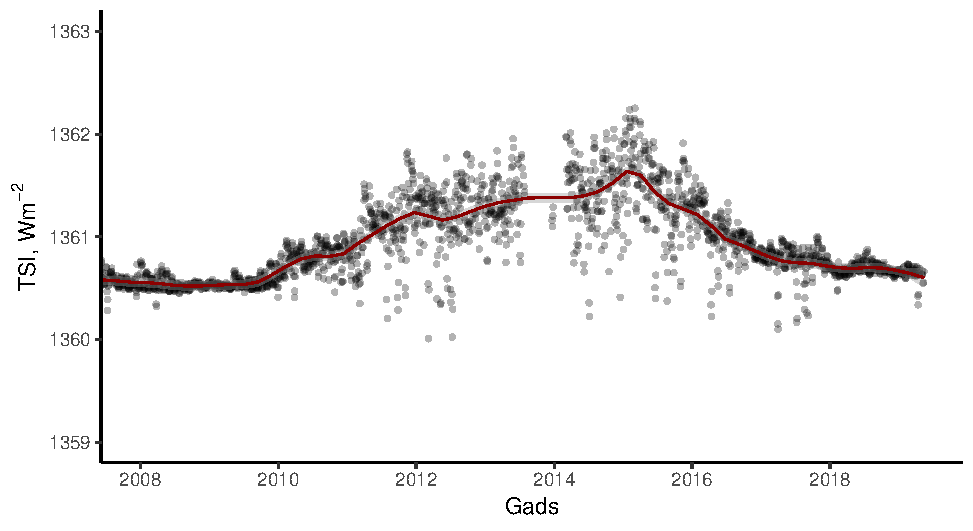
\includegraphics[width=\linewidth]{figures/misc/TSI_8-19.pdf}
    \captionof{figure}{Kopējais saules apstarojums 24. saules ciklā}
    \label{fig:TSI1}
\end{figure}

\begin{figure}
    \centering
    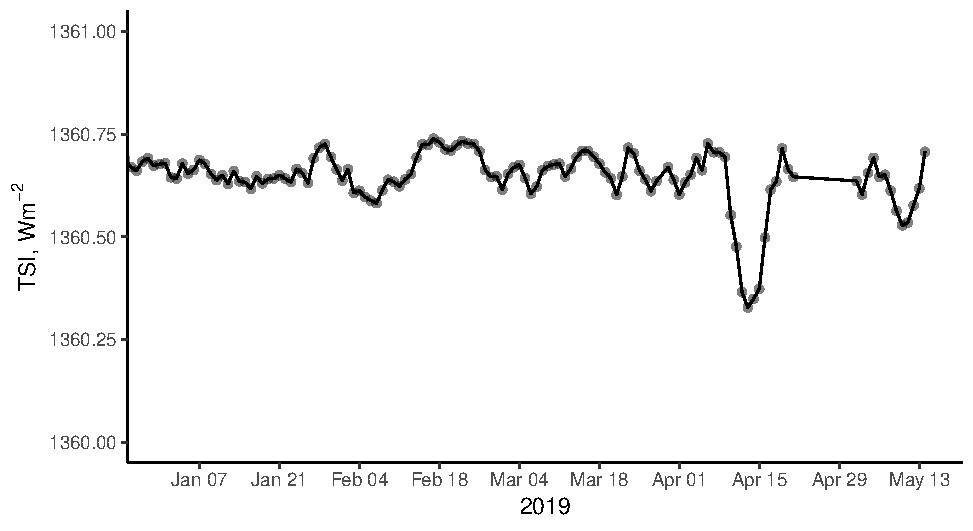
\includegraphics[width=\linewidth]{figures/misc/TSI.pdf}
    \captionof{figure}{Kopējais saules apstarojums solāro paneļu datu ieguves laikā}
    \label{fig:TSI2}
\end{figure}